\section{Design}
In questo capitolo verranno descritti gli aspetti di progettazione sui quali si basa l'elaborato svolto.

\subsection{Struttura}

Per lo sviluppo del sistema è stato scelto di utilizzare un'architettura ibrida tra \emph{Client-Server} e \emph{Peer-to-Peer}. Come si può vedere in figura \ref{fig:architettura} il server sarà il punto di snodo tra i client e il database, svolgendo inoltre la funzione di \emph{discovery server} per quanto riguarda la rete p2p. Ogni client sarà quindi in comunicazione con il server per le funzioni di autenticazione, discovery e interazioni con il database, ma una volta entrato in un \emph{party} sarà connesso direttamente agli altri client. In questo modo il carico di lavoro per il server centrale sarà ridotto al minimo, poiché le informazioni relative alle partite saranno condivise solo all'interno delle reti p2p create. Così facendo si introduce anche un livello di tolleranza in caso di errori all'interno della rete in quanto, dopo aver svolto il ruolo di discovery, ovvero dopo aver inviato gli indirizzi dei peer già presenti all'interno di un party al nuovo peer che fa richiesta di entrarvici e viceversa, se il server dovesse non essere più raggiungibile i peer potrebbero comunque avviare la partita e continuare a giocare perdendo solamente la funzionalità di salvataggio al termine della stessa. Inoltre la singola rete p2p potrà ripristinare lo stato originale della partita nel caso in cui si verifichi il fallimento di più nodi poiché tutti i peer condivideranno uno stato coerente e completo del loro stato.

\begin{figure}[H]
\centering
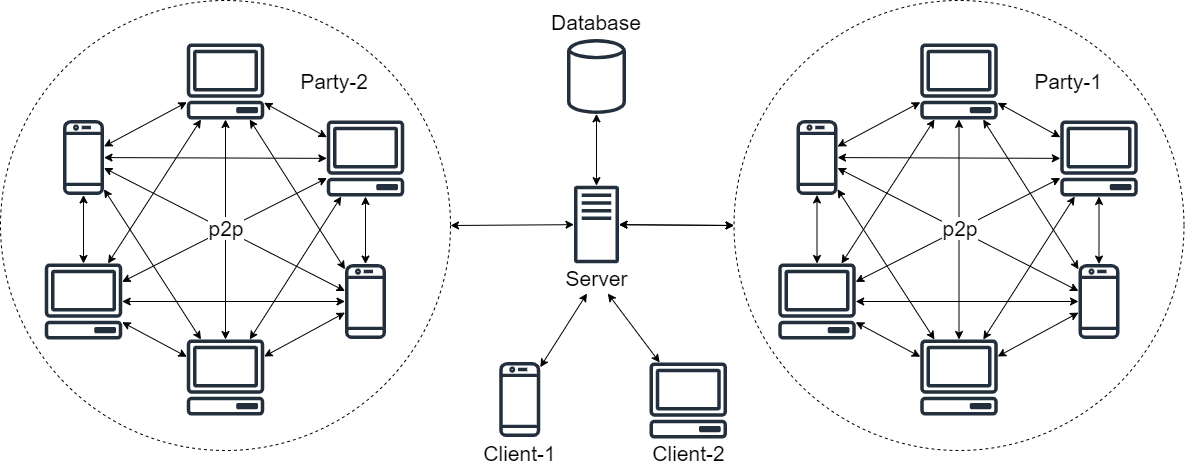
\includegraphics[width=\textwidth]{img/draw/architettura.png}
\caption{Sintesi architettura del sistema}
\label{fig:architettura}
\end{figure}

\subsubsection{Server}
Il server come detto in precedenza si basa sul framework Express, in accordo con lo stack MERN, e svolge il ruolo di \emph{discovery} per i client che si connettono. Sfruttando la libreria Mongoose all'avvio viene effettuata la connessione al database, dopodiché vengono impostate le route per le richieste HTTP e gli handler per i messaggi ricevuti attraverso le web-socket.\\[\baselineskip]\indent
Al fine di evitare una crescita incontrollata delle comunicazioni nel caso il sistema venga scalato a un utilizzo più esteso sono state utilizzate le \emph{rooms} \cite{socketIORooms} messe a disposizione dalla libreria, ovvero dei canali di comunicazione ai quali le socket possono unirsi che permettono al server di inviare messaggi a specifici sottoinsiemi di client senza effettuare broadcast delle informazioni. La singola room corrisponde come concetto a quello di party descritto in precedenza, rappresentando quindi un gruppo di giocatori logicamente isolato dagli altri.

Il server implementato sarà di tipo \emph{stateful}. Alla base di questo stato ci saranno due liste contenenti strutture dati come riportate nelle figure \ref{fig:sessionStorage} e \ref{fig:room}.
Lo stato degli utenti autenticati verrà mantenuto all'interno del campo\emph{sessionStorage}, il quale assocerà a un identificativo univoco utilizzato come chiave, un valore corrispondente alle informazioni di accesso del giocatore, in questo caso \emph{username} e stato di connessione. Le informazioni riguardo la suddivisione in stanze verranno invece memorizzate in una lista di oggetti \emph{room} composti dall'identificativo della stanza stessa, una lista di giocatori, identificati da \emph{username} e \emph{peerId}, e dallo stato di chiusura.

\begin{figure}[H]
    \centering
    \begin{minipage}{0.45\textwidth}
        \centering
        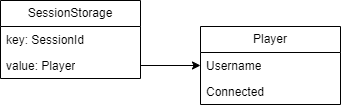
\includegraphics[width=0.9\textwidth]{img/draw/uml_sessionstorage.png}
        \caption{Schema sessione}
        \label{fig:sessionStorage}
    \end{minipage}\hfill
    \begin{minipage}{0.45\textwidth}
        \centering
        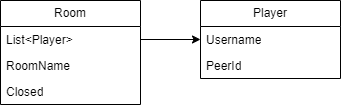
\includegraphics[width=0.9\textwidth]{img/draw/uml_room.png}
        \caption{Schema stanze}
        \label{fig:room}
    \end{minipage}
\end{figure}

\subsubsection{Database}
Il database utilizzato dal sistema è stato strutturato in maniera semplice con l'obiettivo di familiarizzare con le tecnologie impiegate, raggiungendo comunque i requisiti che erano stati prefissati.

Come si può vedere nella figura \ref{fig:dbClasses} le informazioni salvate si riassumono in due classi, \emph{user} e \emph{game}. La prima contiene le informazioni relative al singolo utente, ovvero:
\begin{itemize}
    \item \textbf{username:} nome scelto dall'utente in fase di registrazione, univoco all'interno del database.
    \item \textbf{password:} la password impostata che viene salvata come hash utilizzando la libreria \emph{bcript} \cite{bcryptWikipedia}.
    \item \textbf{goodWins/badWins:} statistiche aggregate relative alle vittorie ottenute in base alla squadra di appartenenza.
    \item \textbf{playedGames:} una lista contenente gli identificativi delle partite giocate dall'utente.
\end{itemize}
Alcune delle informazioni salvate possono essere considerate ridondanti, come ad esempio il campo \emph{playedGames}, ma sono state pensate per uno stato futuro del sistema nel quale il numero di entità di \emph{game} sarà molto elevato, causando così una possibile complessità computazionale crescente per la ricerca di tutte le partite nelle quali ha partecipato uno specifico giocatore.\\
La classe \emph{game} è composta da:
\begin{itemize}
    \item \textbf{gameCode:} codice univoco utilizzato per identificare la partita.
    \item \textbf{winners:} la squadra vincitrice.
    \item \textbf{players:} un array contenente gli username dei giocatori partecipanti e il loro relativo ruolo.
    \item \textbf{history:} un array la "storia" della partita, ovvero tutti i suoi avvenimenti.
\end{itemize}

\begin{figure}[H]
\centering
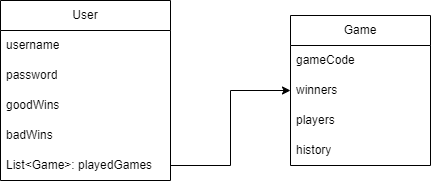
\includegraphics[width=0.5\textwidth]{img/draw/uml_db.png}
\caption{Diagramma delle classi}
\label{fig:dbClasses}
\end{figure}

\subsubsection{Client}
Anche il client rispetta lo stack scelto per il sistema e si basa quindi sul framework React. La sua struttura interna si basa su due macro comportamenti coesistenti, comportandosi come client nei confronti del server centralizzato e come peer nei confronti degli altri client connessi.

\paragraph{Redux}
Per quanto riguarda lo stato del client è stata invece sfruttata la libreria Redux in aggiunta al concetto di stato presente in React. Gli oggetti creati e utilizzati in questo caso, visibili nella figura \ref{fig:reduxClasses}, sono i seguenti:
\begin{itemize}
    \item \textbf{user:} contiene tutte le informazioni relative all'utente.
        \begin{itemize}
            \item \textbf{username:} nome univoco identificativo.
            \item \textbf{room:} il codice identificativo del party selezionato.
            \item \textbf{token:} identificativo della sessione.
            \item \textbf{stats:} contiene le statistiche ricevute dal server.
        \end{itemize}
    \item \textbf{util:} raccolta di booleani utili al sistema per definirne lo stato.
        \begin{itemize}
            \item \textbf{socketConnected:} stato della socket verso il server.
            \item \textbf{peerConnected:} stato della connessione del peer.
            \item \textbf{isLoading:} stato di caricamento, attesa di informazioni.
            \item \textbf{cardVisible:} necessità di mostrare la carta all'avvio della partita.
        \end{itemize}
    \item \textbf{game:} contiene tutte le informazioni relative alla singola partita.
        \begin{itemize}
            \item \textbf{gameCode:} codice univoco generato per identificare la partita.
            \item \textbf{partyClosed:} \emph{True} se il party è completo e chiuso.
            \item \textbf{players:} array dei giocatori in partita.
            \item \textbf{phase:} fase della partita.
            \item \textbf{history:} array contenente lo storico della partita.
            \item \textbf{wolfNumber:} numero di lupi impostati.
            \item \textbf{extras:} informazioni su quali personaggi extra sono stati impostati.
        \end{itemize}
\end{itemize}

\begin{figure}[H]
\centering
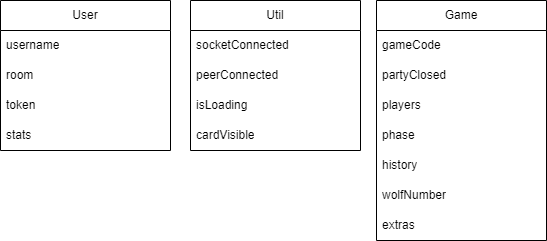
\includegraphics[width=0.8\textwidth]{img/draw/uml_redux.png}
\caption{Diagramma stato di Redux}
\label{fig:reduxClasses}
\end{figure}


\subsubsection{Interfaccia}
Lo sviluppo dell'interfaccia utente è stato effettuato in maniera incrementale consultando amici e colleghi del corso per meglio definire le componenti fondamentali e gli scenari di utilizzo. Dopo una prima fase di bozzetti su carta sono stati disegnati i wireframe del progetto utilizzando Figma. La parte di definizione e implementazione ha poi tenuto conto dei principali criteri di accessibilità.

\paragraph{Wireframe}
Le interfacce sono state sviluppate seguendo il criterio \emph{mobile-first}, qui di seguito verranno riportati esempi di visualizzazione sia mobile che da desktop. Tutte le schermate avranno una \emph{navbar} contenente il logo dell'applicazione e un menu a tendina che potrà contenere diverse funzionalità a seconda dello stato del sistema.\\[\baselineskip]\indent
La prima schermata che si presenterà all'utente sarà quella di accesso, visibile nelle figure \ref{fig:pcLogin} e \ref{fig:androidLogin}, dalla quale sarà possibile registrarsi inserendo delle nuove credenziali o accedere attraverso quelle inserite in precedenza.

\begin{figure}[H]
\centering
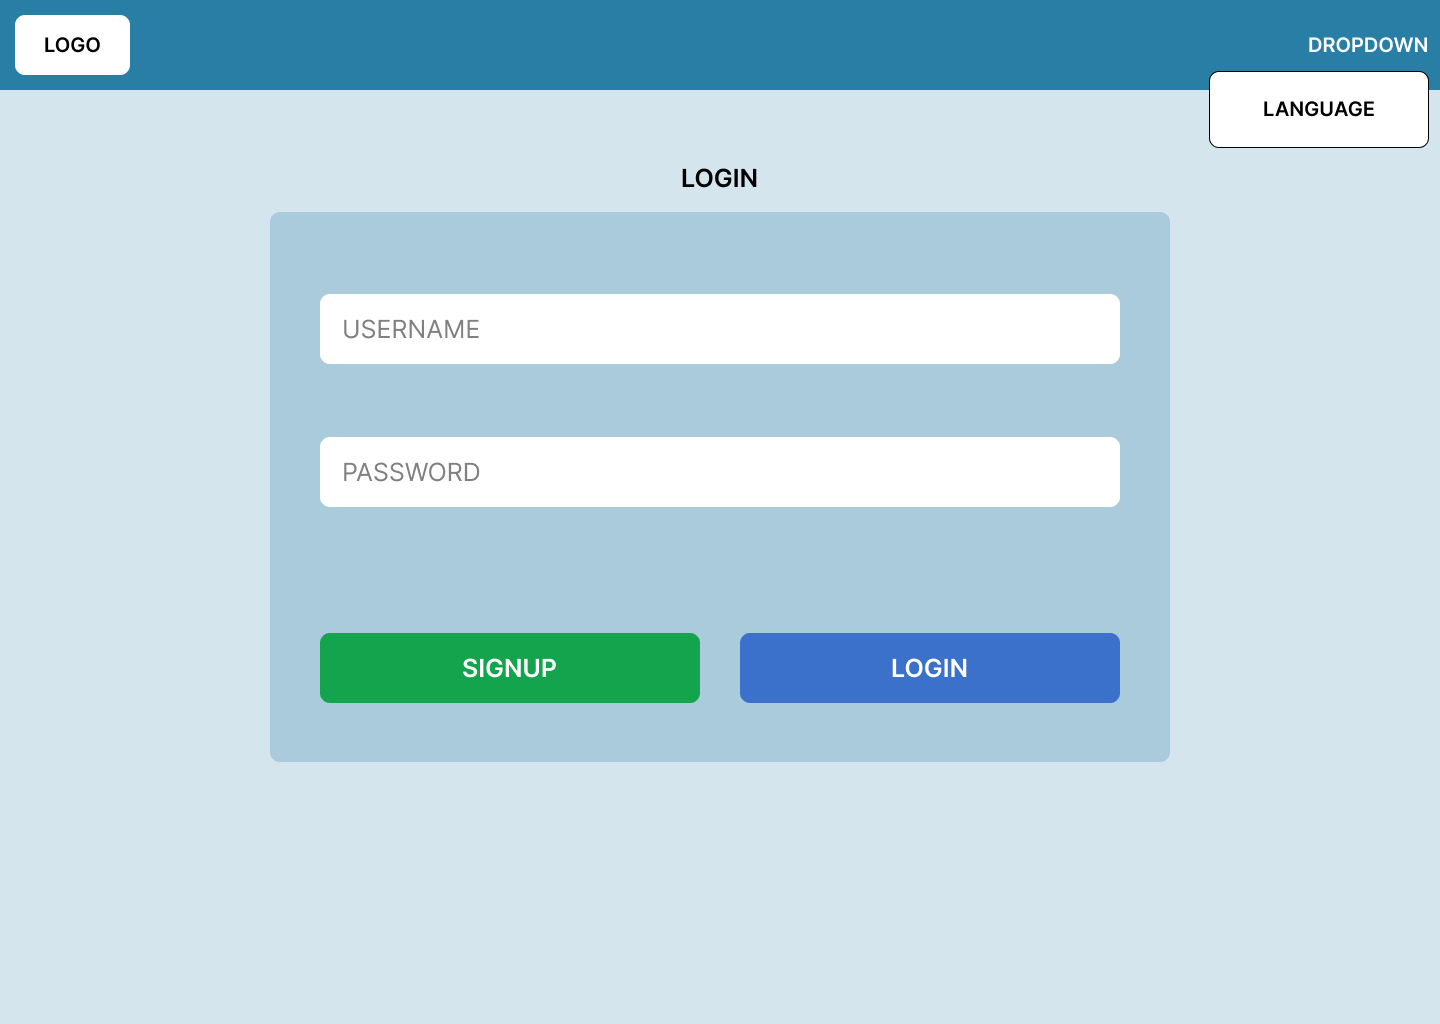
\includegraphics[width=0.6\textwidth]{img/figma/Wireframe-1.png}
\caption{Schermata di login}
\label{fig:pcLogin}
\end{figure}


A seguire una volta effettuato il login l'utente potrà inserire un codice identificativo di una room da creare o alla quale unirsi, attraverso un form visibile nella figura \ref{fig:pcRoom}. Nella stessa figura è mostrata come esempio anche una notifica che il sistema potrà mandare all'utente sfruttando la libreria \emph{react-notifications}\cite{npmjsReactnotifications}.

\begin{figure}[H]
\centering
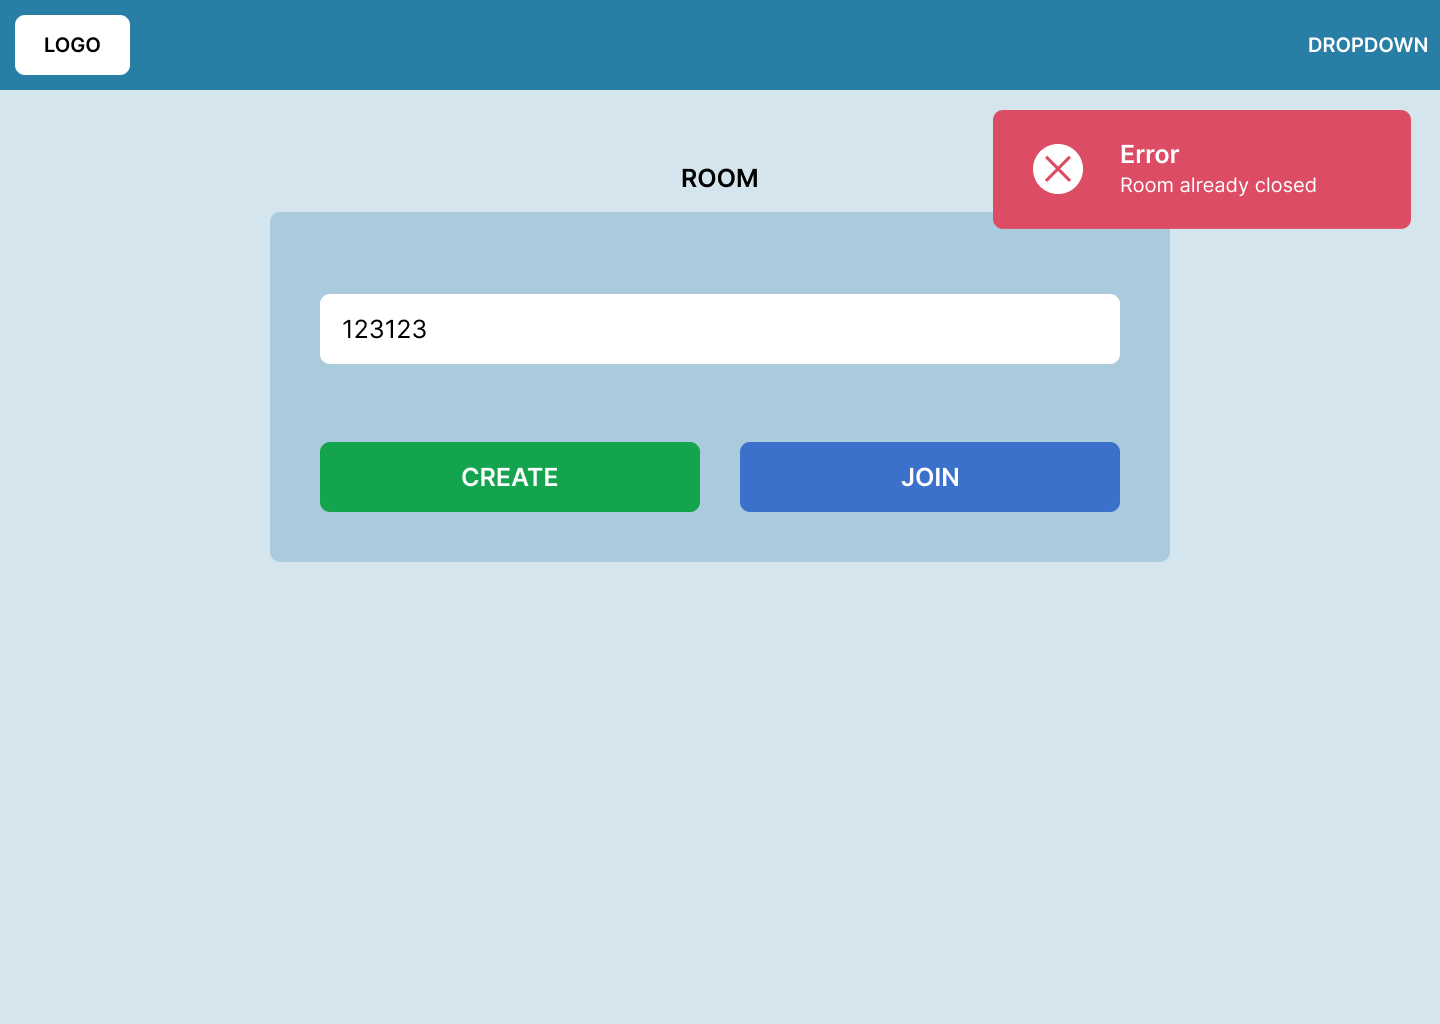
\includegraphics[width=0.6\textwidth]{img/figma/Wireframe-2.png}
\caption{Schermata di selezione della room}
\label{fig:pcRoom}
\end{figure}

Una volta all'interno all'utente verrà mostrata una schermata come quella in figura \ref{fig:pcLobby} nella quale si avrà la possibilità di chiudere la room una volta raggiunto il numero minimo di giocatori richiesto. Successivamente in base alle specifiche di implementazione del gioco sarà data la possibilità attraverso un modale di modificare le impostazioni di gioco, come il numero di lupi o eventuali personaggi extra che si vogliono utilizzare.

\begin{figure}[H]
\centering
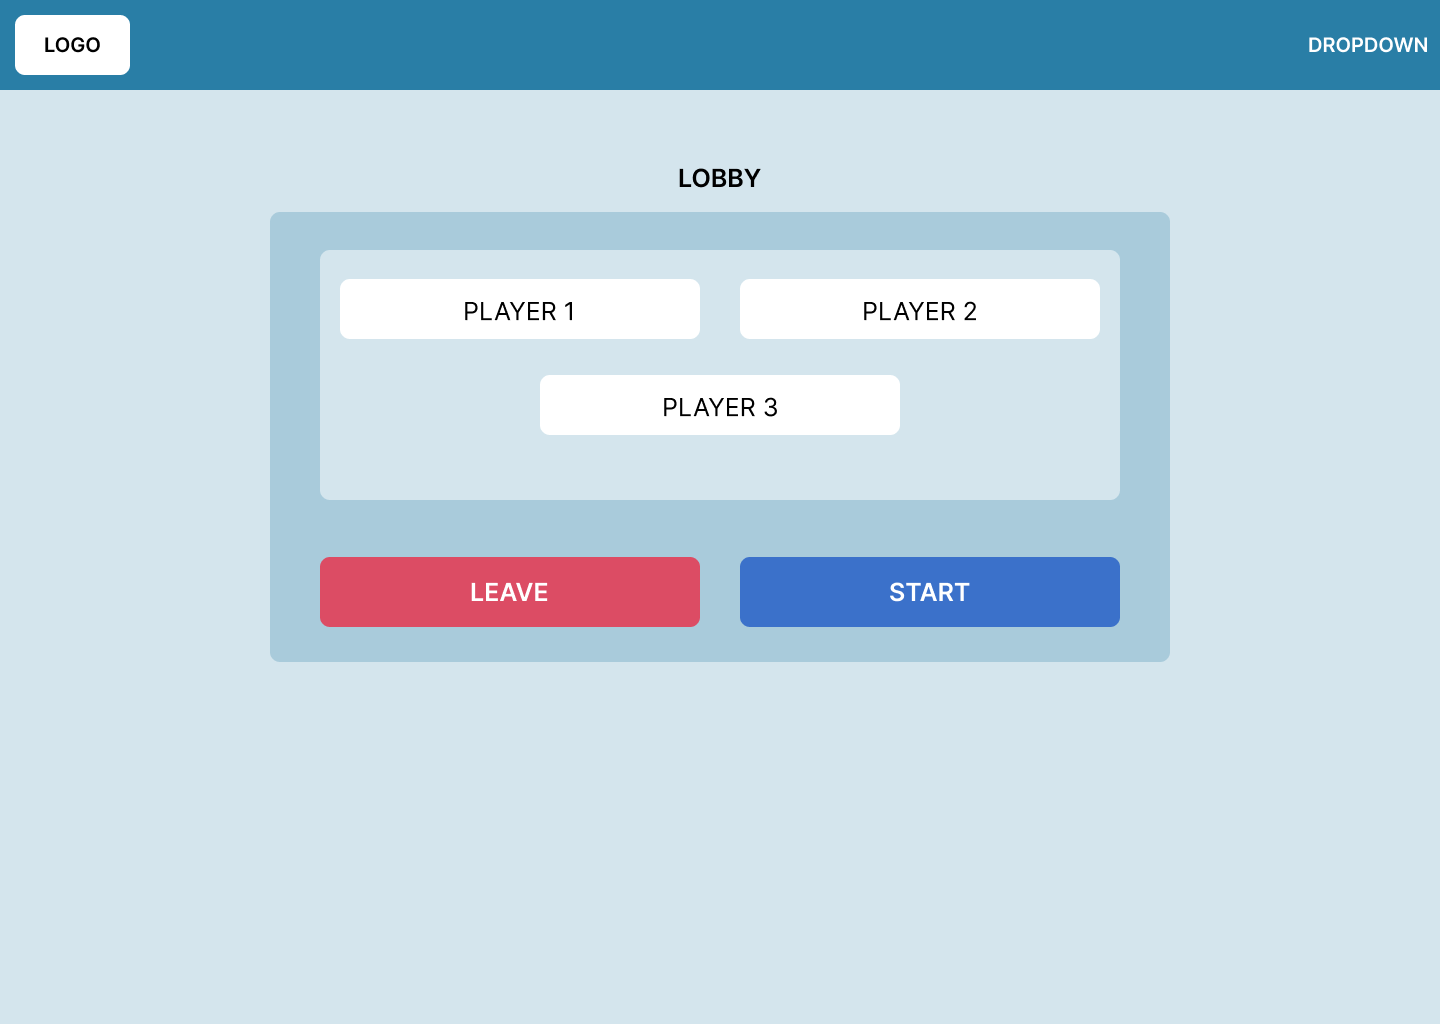
\includegraphics[width=0.6\textwidth]{img/figma/Wireframe-3.png}
\caption{Schermata interna alla room}
\label{fig:pcLobby}
\end{figure}

Dopo aver avviato la partita la schermata di gioco sarà quella mostrata nella figura \ref{fig:pcGame}, strutturata su tre colonne contenenti le informazioni necessarie, l'elenco dei giocatori partecipanti, la carta rappresentante il ruolo del giocatore e lo storico degli avvenimenti della partita. In base alla fase di gioco nella parte alta della schermata verrà poi mostrato un ulteriore elenco dei giocatori tra i quali scegliere chi si vuole votare. Nella visualizzazione mobile mostrata nella figura \ref{fig:androidGame} le colonne verranno disposte verticalmente in maniera reattiva in base alla dimensione della finestra.

\begin{figure}[H]
\centering
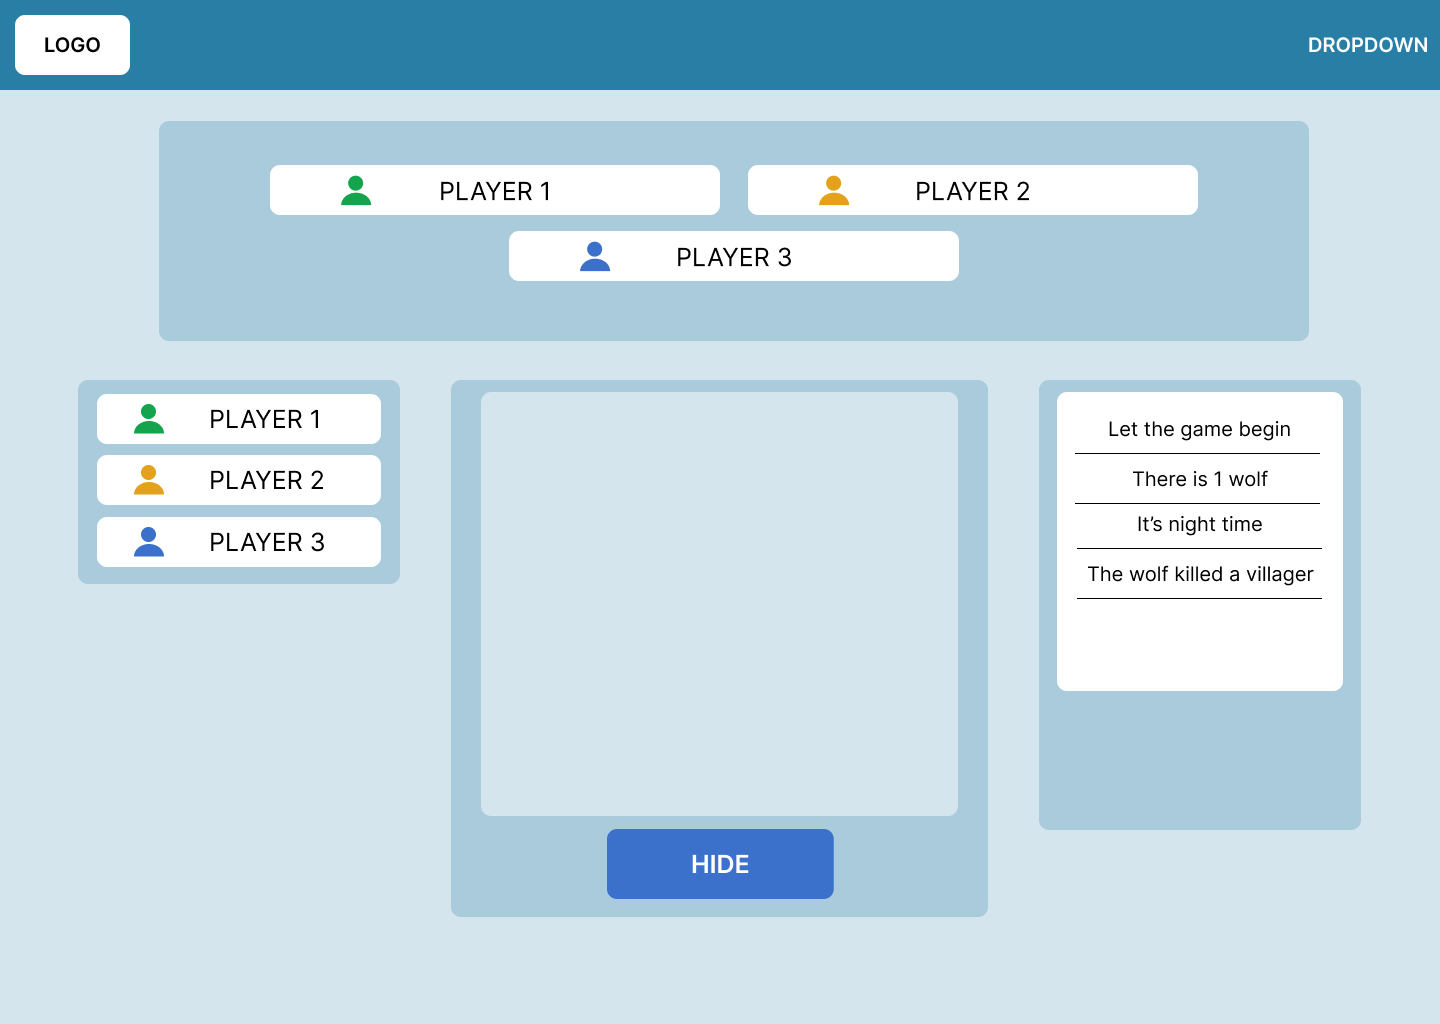
\includegraphics[width=0.6\textwidth]{img/figma/Wireframe-4.png}
\caption{Schermata di gioco}
\label{fig:pcGame}
\end{figure}


\begin{figure}[H]
    \centering
    \begin{minipage}{0.45\textwidth}
        \centering
        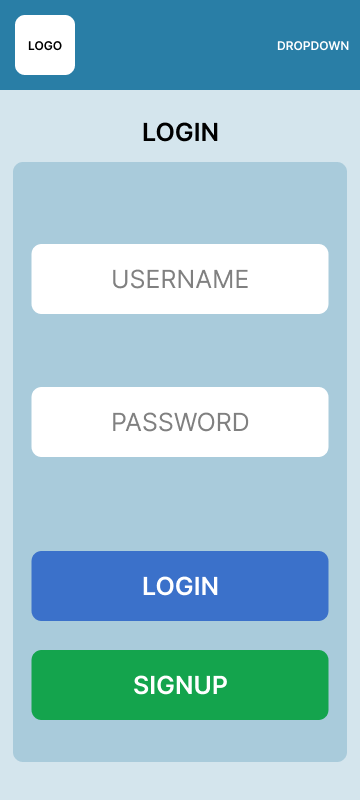
\includegraphics[width=0.5\textwidth]{img/figma/AndroidLarge-1.png} \caption{Schermata di login per dispositivo mobile}
        \label{fig:androidLogin}
    \end{minipage}\hfill
    \begin{minipage}{0.45\textwidth}
        \centering
        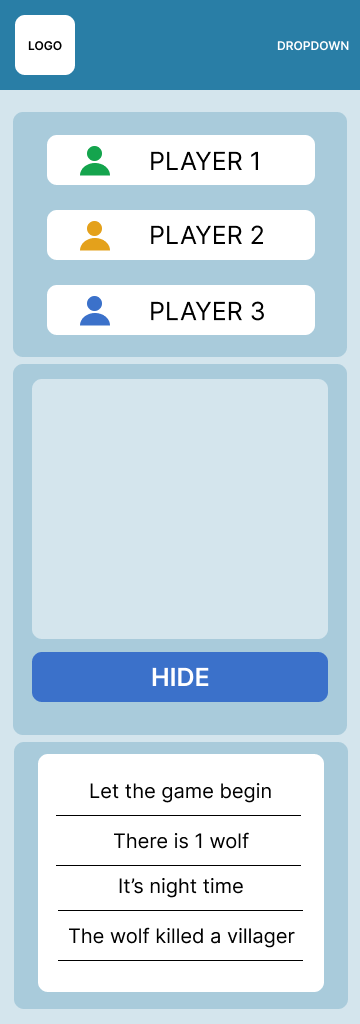
\includegraphics[width=0.5\textwidth]{img/figma/AndroidLarge-2.png} \caption{Schermata di gioco per dispositivo mobile}
        \label{fig:androidGame}
    \end{minipage}
\end{figure}

\subsection{Comportamento}

In questa sezione si descriverà sinteticamente il comportamento delle due parti principali del sistema.

\subsubsection{Server}
Qui di seguito nella figura \ref{fig:serverStates} viene riportato il diagramma degli stati che il server attraversa durante la sua esecuzione. Una volta avviato, dopo una fase di inizializzazione e import, il server effettuerà un tentativo di collegamento al database. Nel caso dovesse fallire l'esecuzione viene terminata in quanto non è prevista la possibilità di utilizzare il sistema senza un database.

Una volta effettuata la connessione e impostati gli handler il server si mette in ascolto sulla porta 8080, se non diversamente specificato in fase di avvio.

Raggiunto questo stato che può essere considerato finale il server si occuperà soltanto di ricevere messaggi dai client, elaborare la risposta, aggiornando se necessario il proprio stato interno, per poi inviarla al mittente oppure come messaggio di broadcast a seconda delle necessità.


\begin{figure}[H]
\centering
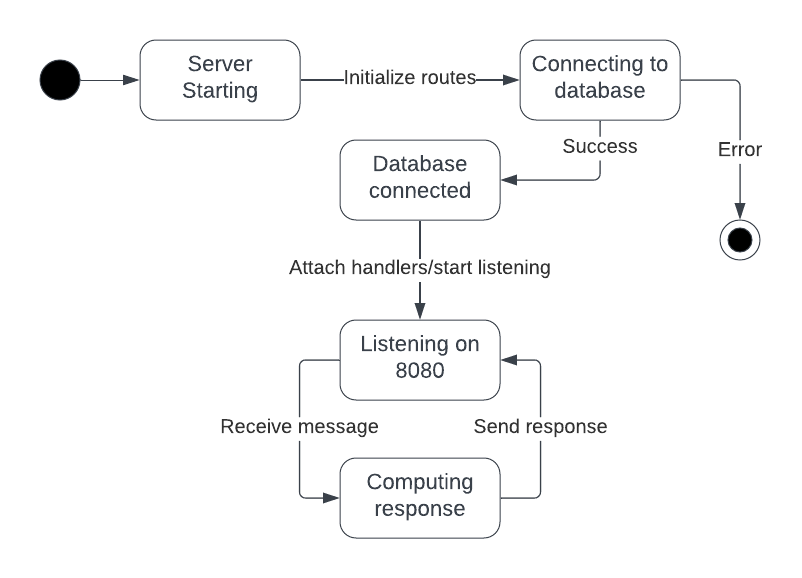
\includegraphics[width=0.7\textwidth]{img/draw/uml_state_server.png}
\caption{Diagramma degli stati del server}
\label{fig:serverStates}
\end{figure}

\subsubsection{Client}
La figura \ref{fig:clientStates} riporta invece i possibili stati del client. Si può osservare come all'avvio il client non effettui immediatamente il collegamento al server, bensì come attenda la prima azione, che può essere quella di autenticarsi o di registrarsi come nuovo utente, per effettuare il primo tentativo. Nel caso in cui il collegamento dovesse fallire il sistema ritornerebbe allo stato di partenza senza interrompere l'esecuzione.

Una volta effettuata la connessione e l'autenticazione lo stato interno del client viene aggiornato con le nuove informazioni ottenute. Successivamente selezionando il codice di una stanza il client entrerà in uno stato di inizializzazione necessario per avviare la sua componente \emph{peer}. Una volta andata a buon fine la procedura il client nello stato di \emph{lobby} attenderà la chiusura della stessa per passare alla fase di gioco effettiva. A questo punto una volta definita la composizione del party ci sarà un alternarsi di due stati, impostazione dei settaggi di gioco e gioco effettivo, nei quali ogni modifica effettuata dall'utente verrà inviata a tutti gli altri peer connessi e analogamente rimarrà in ascolto per ogni modifica della quale può essere notificato.


\begin{figure}[H]
\centering
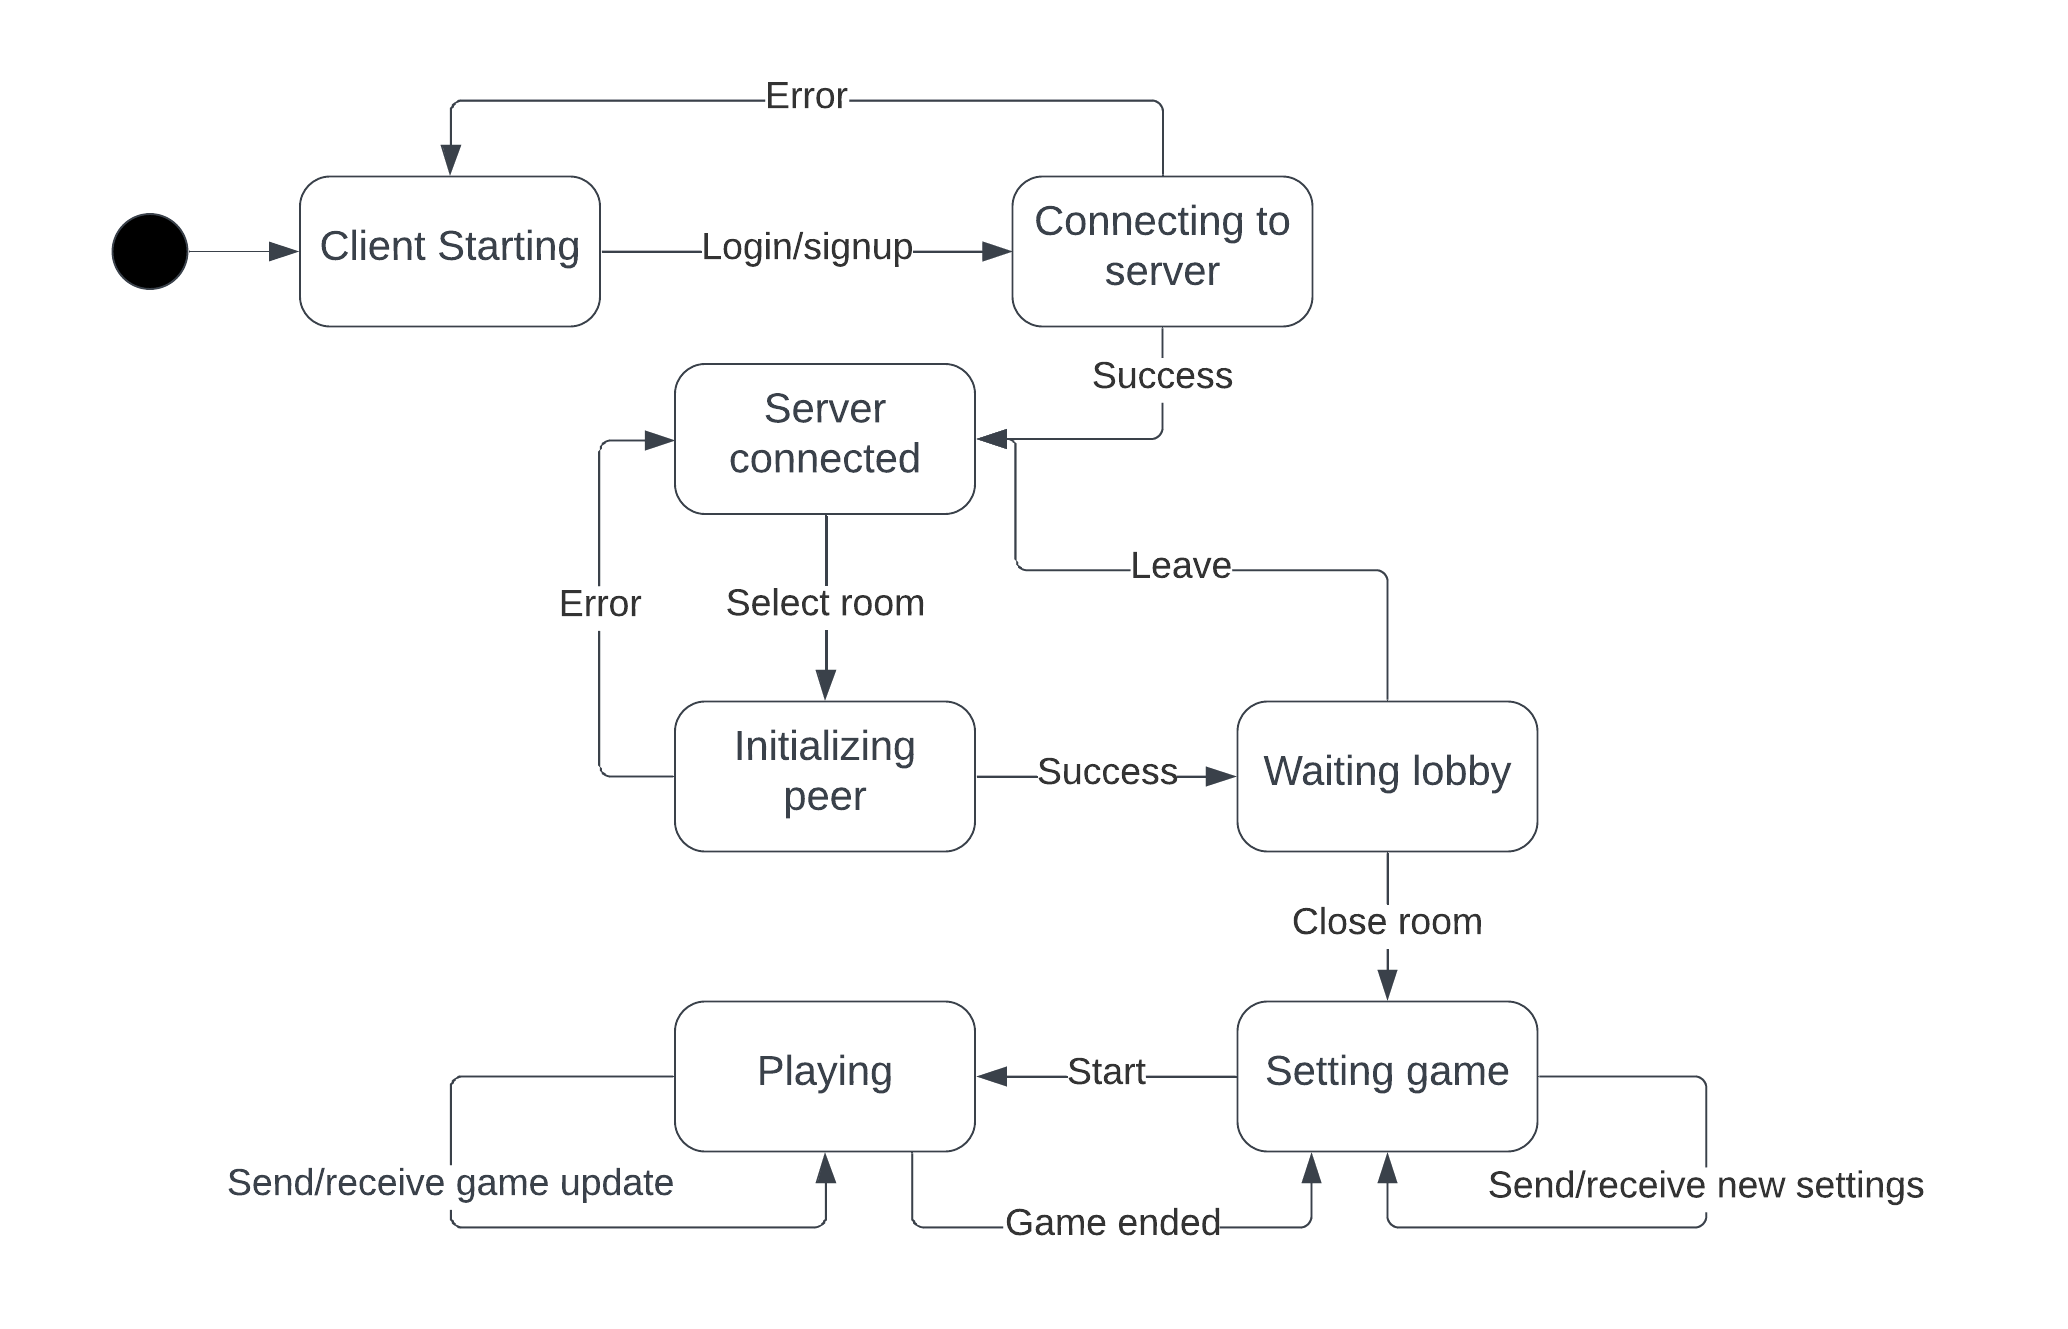
\includegraphics[width=0.9\textwidth]{img/draw/uml_state_client.png}
\caption{Diagramma degli stati del client}
\label{fig:clientStates}
\end{figure}

\subsection{Interazione}

Le interazioni tra i componenti che verranno descritte qui di seguito sono quella tra un client e il server, analizzando quindi la procedura di autenticazione, e quella tra due peer durante le fasi di gioco. È stato ritenuto superfluo approfondire l'interazione tra il server e il database in quanto triviale nella sua implementazione.

\subsubsection{Client-Server}
L'interazione tra client e server avrà inizio nel momento in cui l'utente attraverso l'interfaccia effettuerà la registrazione o l'accesso al sistema.
Nell'esempio riportato in figura \ref{fig:clientServerSequence} viene riportata l'interazione tra le due parti del sistema ipotizzando uno scenario di utilizzo standard.

La connessione alla socket del server viene richiesta dal client nel momento in cui invia il primo messaggio, che può essere di \emph{signup} o \emph{login}. Il server invia poi in risposta all'accesso la sessione dell'utente, la quale viene anche memorizzata per permettere di ristabilire la connessione in caso di fallimenti.

Il client può poi richiedere le statistiche relative all'utente che saranno inviate in risposta dal server.

Per procedere all'inizio del gioco il client invierà un messaggio \emph{room} contenete l'identificativo della lobby nella quale vuole entrare, dopodiché, in caso il codice non corrisponda a una stanza già chiusa nella quale non si era presenti in precedenza, il server invierà un messaggio di conferma al client stesso.
A livello di comunicazione il codice della room verrà poi utilizzato per identificare un canale, indicato come \emph{:Room} in figura, sul quale verrà effettuata una broadcast a tutti i client già connessi comunicando l'ingresso di un nuovo peer. Analogamente al client verranno inviate le informazioni di tutti i peer già presenti.

Nel momento in cui il client comunica al server di voler chiudere la room viene anche in questo caso effettuata una broadcast allo specifico canale.
Da questo punto in poi le interazioni tra client e server si sospendono, e hanno inizio le interazioni di gioco che saranno descritte nella sezione successiva.
Infine terminata la partita il client potrà comunicare al server la volontà di salvarla nel database

Nel caso in cui un utente lasciasse la partita prematuramente allora verrà comunicata la distruzione del peer al server che si occuperà di notificare il canale. L'ultima interazione mostrata è quella di logout, la quale ha come obiettivo quello di comunicare al server di cancellare le informazioni relative alla sessione dell'utente.

\begin{figure}[H]
\centering
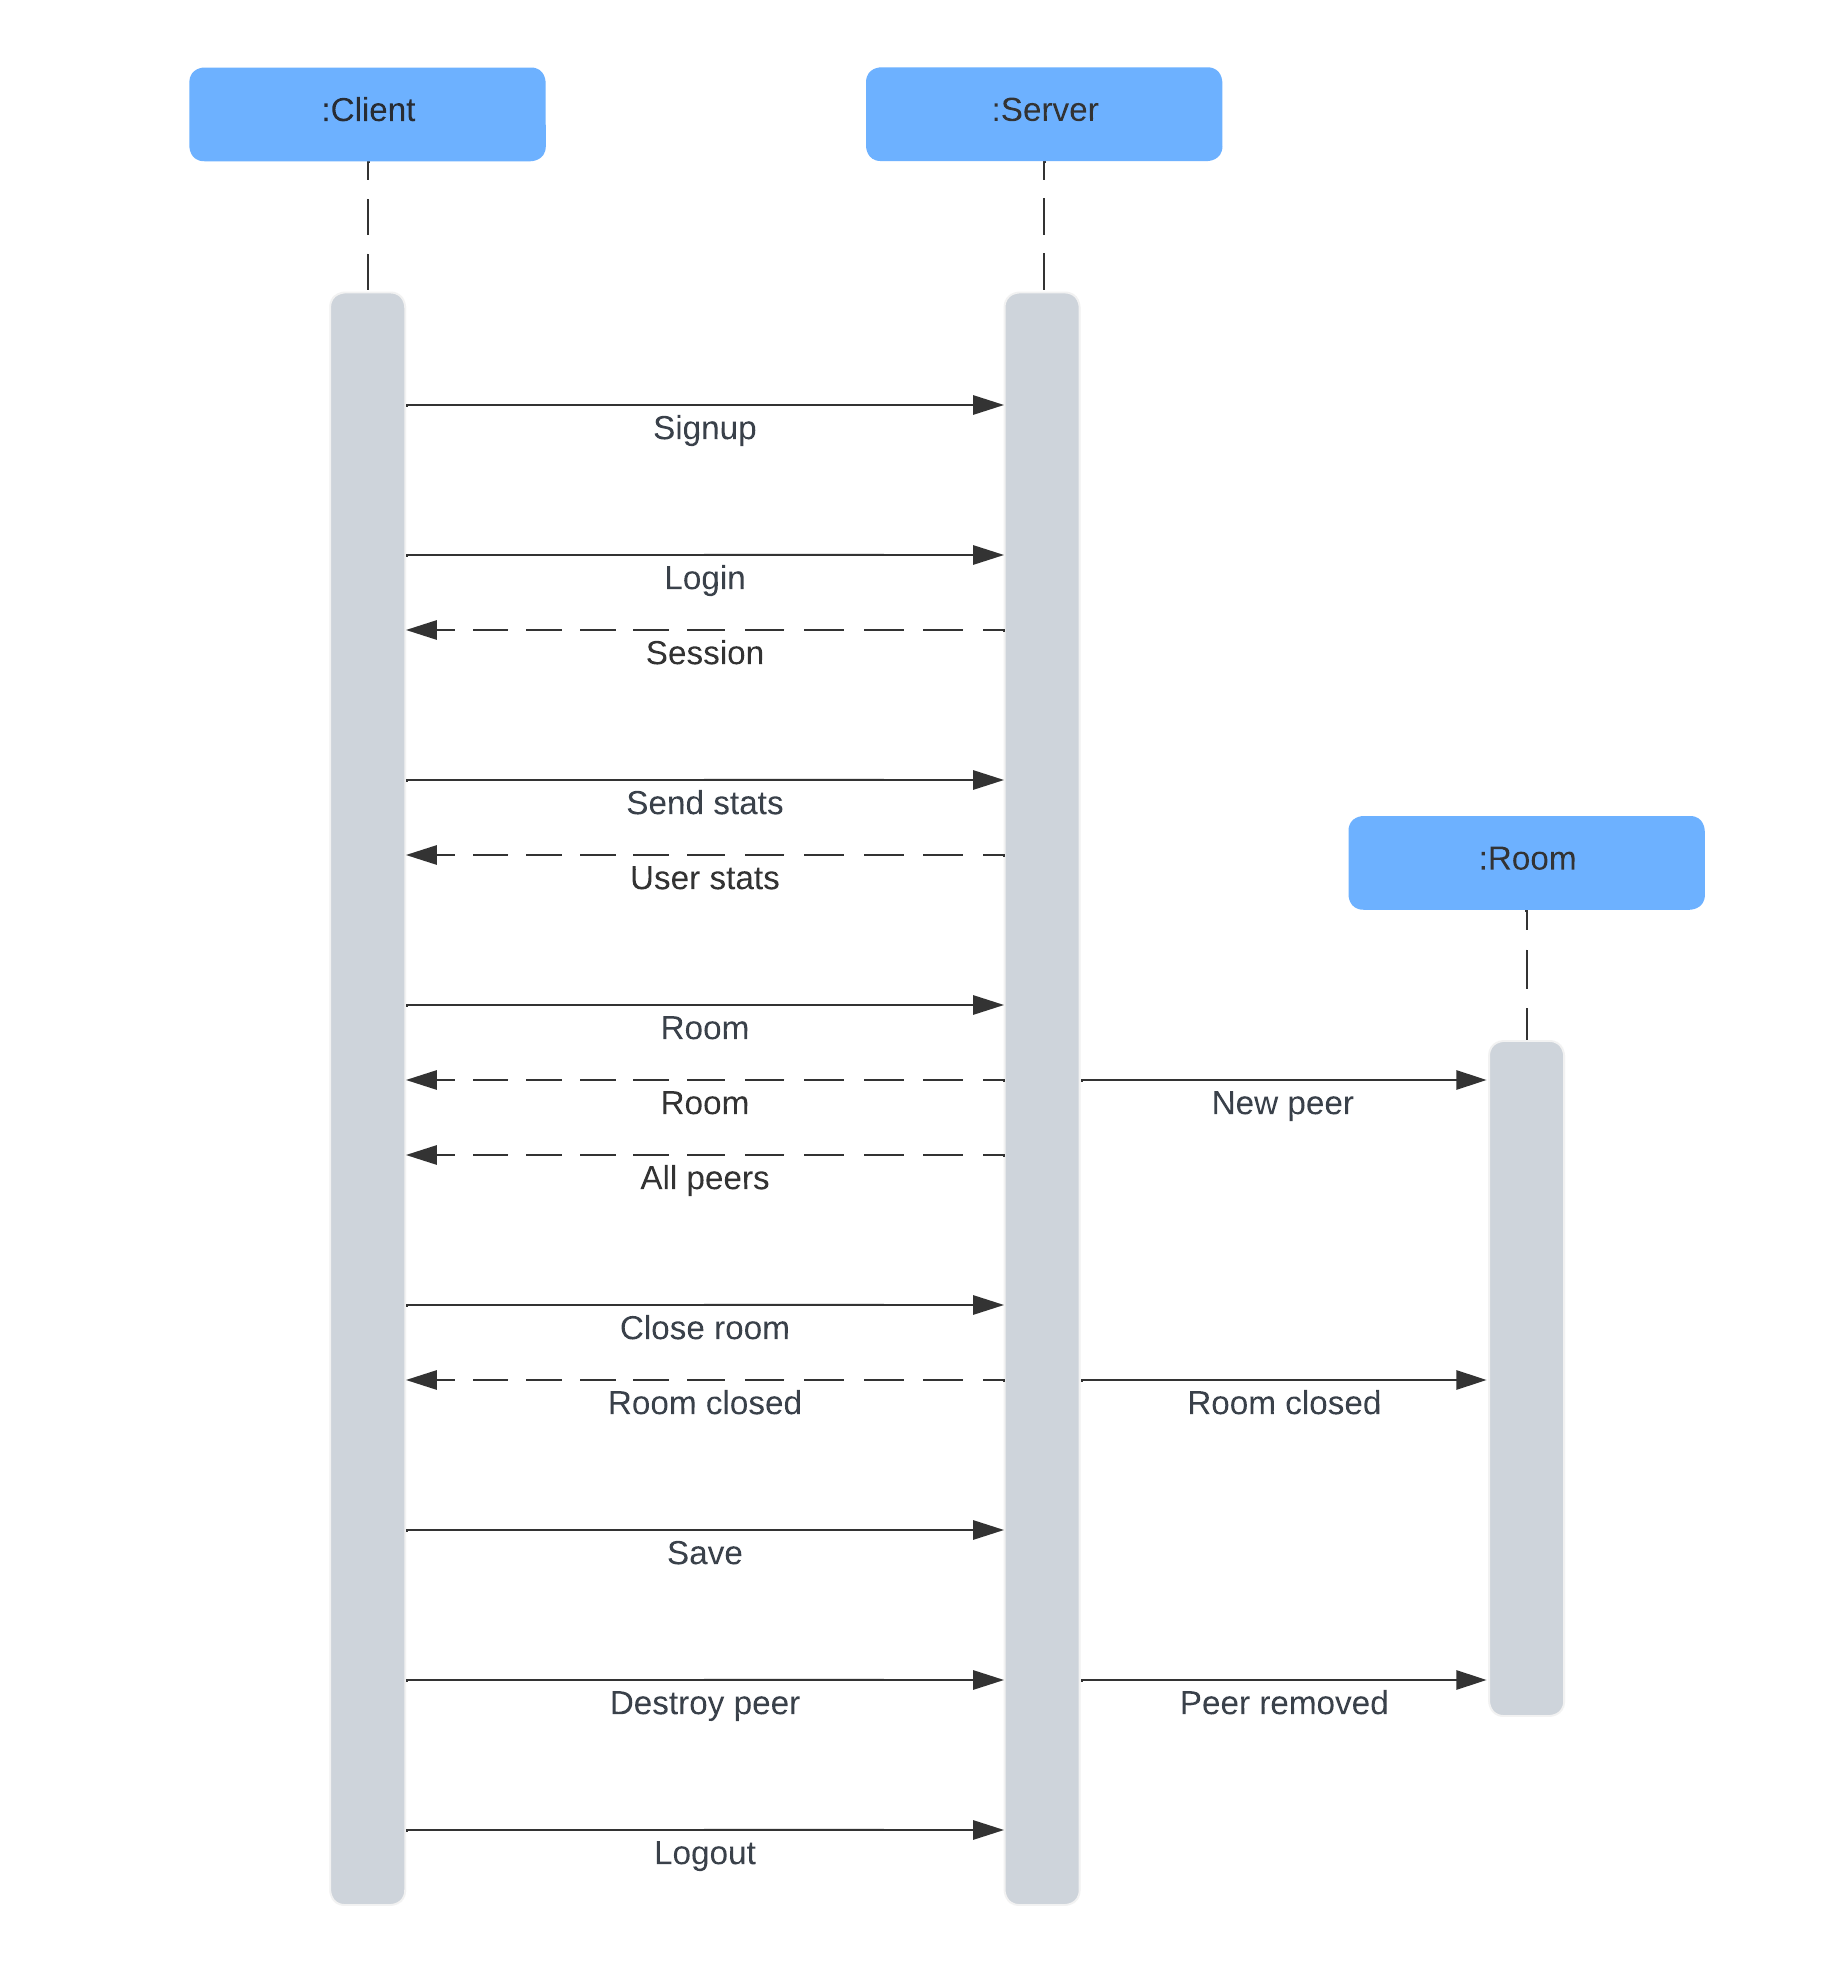
\includegraphics[width=0.83\textwidth]{img/draw/uml_sequence_client_server.png}
\caption{Diagramma di sequenza client-server}
\label{fig:clientServerSequence}
\end{figure}


\subsubsection{Peer-to-Peer}
L'interazione tra i peer è limitata alle fasi di gioco. Nella figura \ref{fig:peerToPeerSequence} è stata riportata una traccia di riferimento semplificata che include nell'insieme \emph{Client-Server} anche l'ultima parte dell'interazione illustrata in precedenza. Si può notare che per mantenere una maggior chiarezza nella figura è stato scelto di rappresentare solo due nodi \emph{Peer\_1} e \emph{Peer\_2} all'interno della rete, nonostante le comunicazioni vengano inviate in modalità broadcast per una più rapida diffusione dell'informazione.

 La prima delle fasi visibile nell'insieme \emph{P2P} è quella di selezione delle impostazioni di gioco, durante la quale le informazioni saranno mantenute coerenti tra i peer inviando messaggi a ogni altro partecipante alla stanza per tutte le modifiche effettuate. Una volta effettuate le modifiche necessarie sarà sufficiente cliccare sul bottone di avvio della partita per generare e successivamente inviare il \emph{GameCode}, entrando così nell'insieme \emph{Game} delle comunicazioni.

 In questa parte di gioco in base al ruolo del partecipante potrà essere chiesto di effettuare una votazione, la quale verrà condivisa con gli altri utenti attraverso l'invio della lista di giocatori \emph{Players} aggiornata con il proprio voto. Seguendo la logica del gioco contestualmente all'ultimo voto della fase verranno inviati anche due messaggi ulteriori, uno per indicare la fase successiva e uno per aggiornare lo storico degli avvenimenti della partita. Questi messaggi raccolti nell'insieme \emph{Game} verranno ripercorsi ciclicamente fino alla vittoria di una delle due parti, segnata dall'invio del passaggio alla fase conclusiva.

 A questo punto tutti i peer avranno la possibilità di inviare le informazioni della partita al server per salvarle sul database in maniera univoca utilizzando il codice generato all'inizio. 
 Con questo messaggio si chiude l'insieme \emph{Game Loop} che può essere percorso nuovamente mantenendo l'insieme di giocatori definito prima della chiusura della stanza.

 Oltre alle comunicazioni illustrate fin'ora può risultare interessante sottolineare una funzione specifica implementata per l'invio cumulativo di tutte le informazioni della partita fino a quel momento, studiata per permettere a un utente di rientrare in gioco in caso di fallimento del sistema. Questa funzione a differenza delle altre interazioni invia i messaggi solo al singolo peer in fase di riconnessione e non in broadcast a tutti i nodi come per gli altri

\begin{figure}[H]
\centering
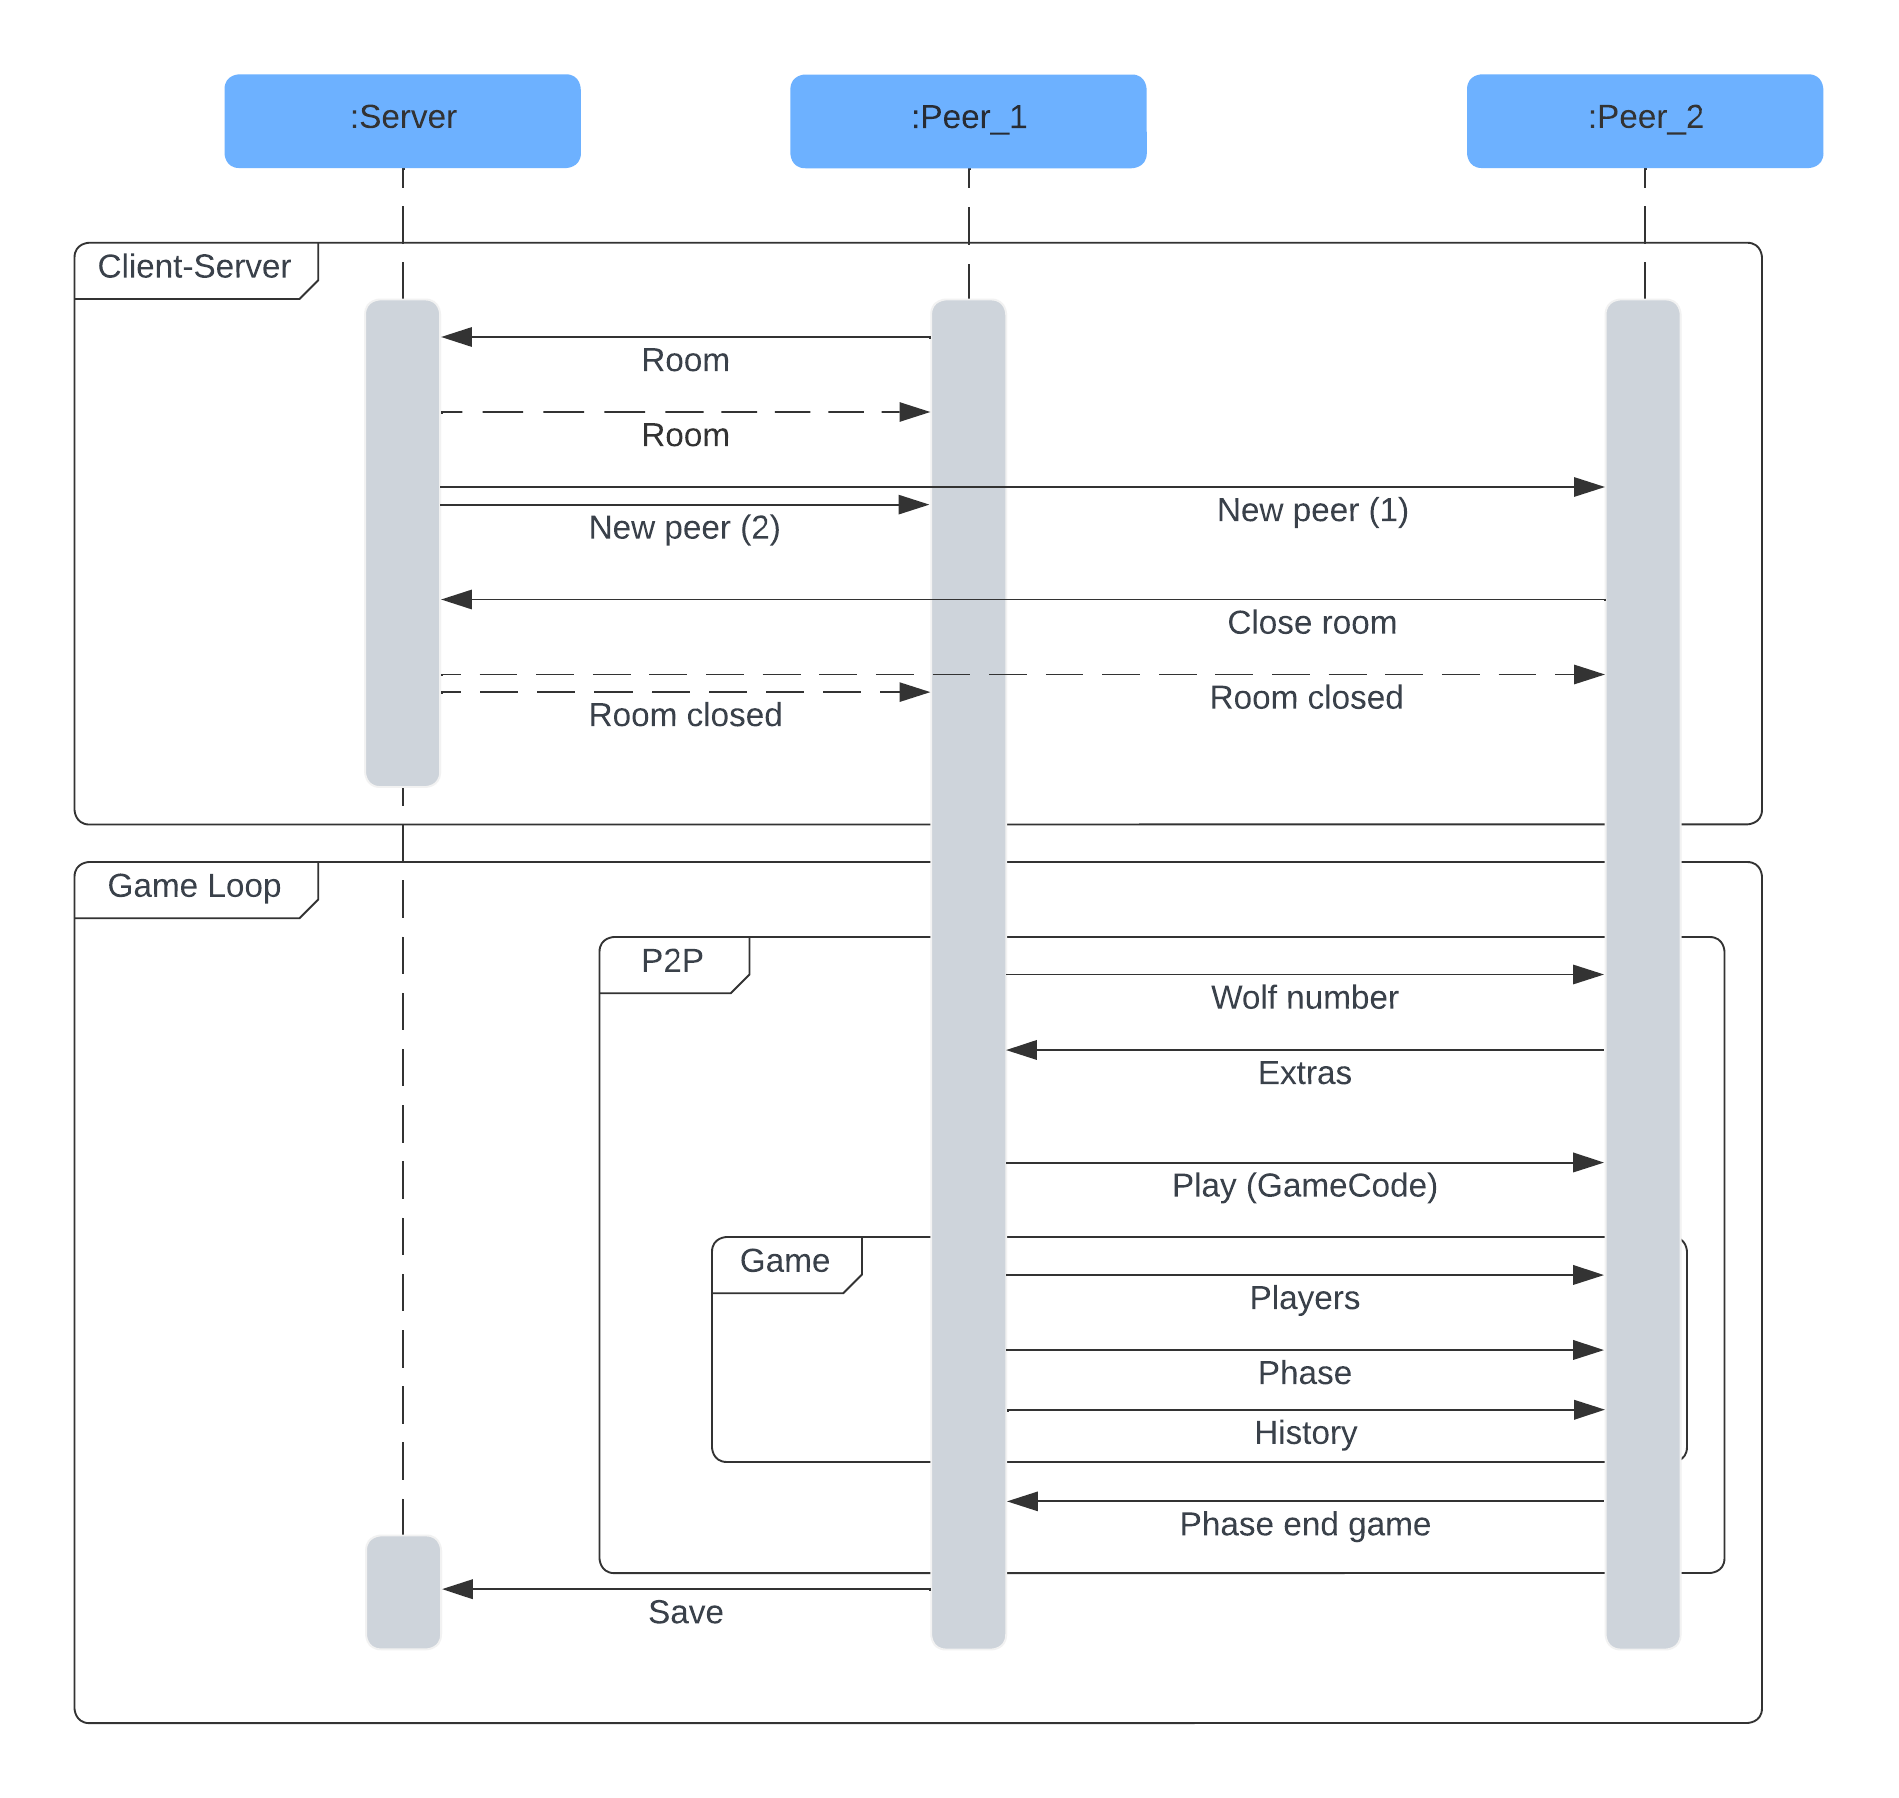
\includegraphics[width=0.83\textwidth]{img/draw/uml_sequence_peer_to_peer.png}
\caption{Diagramma di sequenza peer-to-peer}
\label{fig:peerToPeerSequence}
\end{figure}

